%%%%%%%%%%%%%%%%%%%%%%%%%%%%%%%%%%%%%%%%%
% Beamer Presentation
% LaTeX Template
% Version 1.0 (10/11/12)
%
% This template has been downloaded from:
% http://www.LaTeXTemplates.com
%
% License:
% CC BY-NC-SA 3.0 (http://creativecommons.org/licenses/by-nc-sa/3.0/)
%
%%%%%%%%%%%%%%%%%%%%%%%%%%%%%%%%%%%%%%%%%

%----------------------------------------
%	PREAMBLE
%----------------------------------------

\documentclass{beamer}
\beamertemplatenavigationsymbolsempty
\usepackage{graphicx} % Allows including images
\usepackage{booktabs} % Allows the use of \toprule, \midrule and \bottomrule in tables
% \usepackage[backend=biber,style=apa,citestyle=authoryear]{biblatex}
% \addbibresource{ShippingEmissionsBibDB.bib}
\usepackage{gensymb}
\usepackage{xcolor}
\usepackage{amsmath}
\usepackage{mathtools}
\usepackage{amssymb}
\usepackage{amsfonts}
\usepackage{bbm}

\usetheme{Frankfurt}
% \useoutertheme{trigon}
% \useoutertheme{metropolis}
\setbeamertemplate{itemize items}[circle]
\setbeamertemplate{enumerate items}[default]
\definecolor{UBCblue}{rgb}{0.04706, 0.13725, 0.26667}
\usecolortheme[named=UBCblue]{structure}
\graphicspath{{images/shared}{images/Shipping_Emissions_Introduction}}

\newcounter{saveenumi}
\newcommand{\seti}{\setcounter{saveenumi}{\value{enumi}}}
\newcommand{\conti}{\setcounter{enumi}{\value{saveenumi}}}
\resetcounteronoverlays{saveenumi}

%----------------------------------------------------------
%	TITLE PAGE
%----------------------------------------------------------

\title[]{Shipping Emissions Introduction}

\author{Allen Peters}
\institute[UBC]{
Vancouver School of Economics, University of British Columbia \\
\medskip
\textit{apeters@protonmail.com}
}
\date{\today}

\begin{document}

\begin{frame}
\titlepage
\end{frame}

%------------------------------------------------------

\begin{frame}
\frametitle{Contents}
    \tableofcontents
\end{frame}

%------------------------------------------------------

\section{Intro}

%------------------------------------------------------

\begin{frame}
\frametitle{Motivation}
\begin{itemize}
\setlength{\itemsep}{0.9\baselineskip}
	\item Oceanic shipping contributes $\sim3\%$ of global GHG emissions %, with demand for shipping expected to grow with increasing trade
	\item IMO ranks $\sim$6th as a country
    \item Target of 50\% reduction by 2050
	\item No technological 'silver bullet' 
    \begin{itemize}
        \item Alternative fuels have drawbacks and are undeveloped
    \end{itemize}
\end{itemize}
\end{frame}

%------------------------------------------------------

\setbeamertemplate{caption}{\raggedright\insertcaption\par}
\begin{frame}
\frametitle{Shipping Emissions}
\begin{columns}
	\begin{column}{0.5\textwidth}
        \begin{enumerate}
        \setlength{\itemsep}{0.9\baselineskip}
            \item Container ships:
            \begin{itemize}
                \item Manufactured goods
                \item Concentrated
                \item Fixed routes
            \end{itemize}
            \item Bulk carriers:
            \begin{itemize}
                \item Iron ore, coal, grain...
                \item Unconcentrated
                \item Operate like taxis
                \item Size categories/markets: Handysize, Handymax, Panamax, Capesize
            \end{itemize}
            \item \color{gray}Oil tankers
            \begin{itemize}
                \item 'In-between'
                \item Don't have tracking data
            \end{itemize}
        \end{enumerate}
	\end{column}
	\begin{column}{0.5\textwidth}
		\begin{figure}
			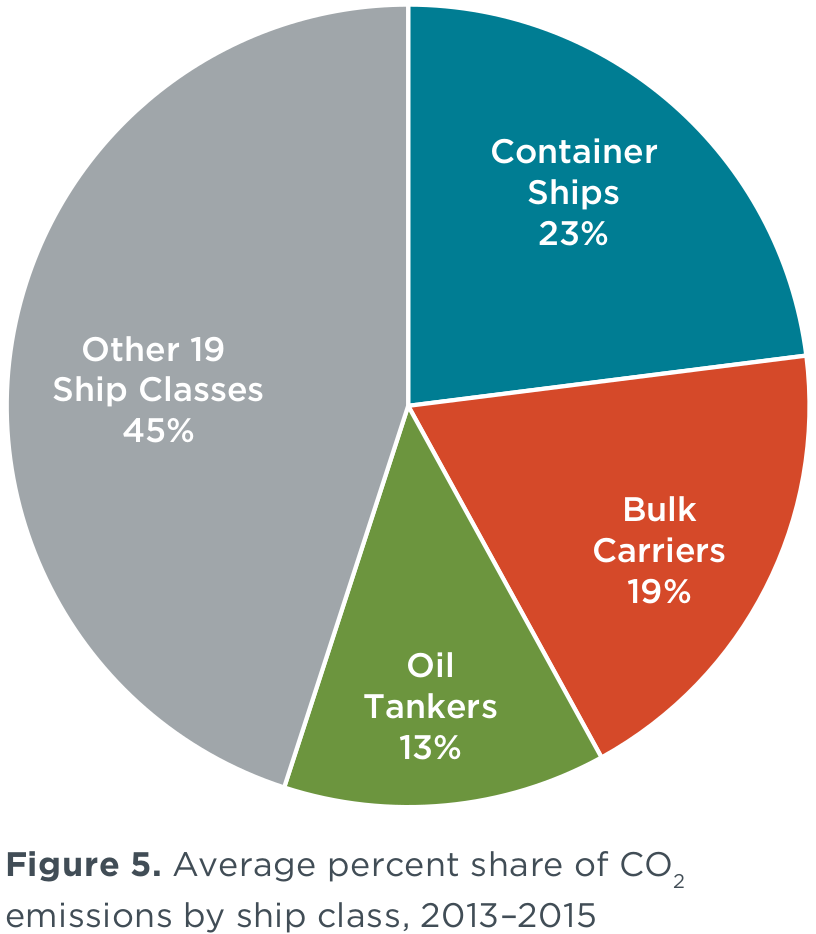
\includegraphics[width = \textwidth]{ICCT_emissions_ship_type.png}
            \caption{Olmer et al. 2017}
		\end{figure}
	\end{column}
\end{columns}
\end{frame}

%------------------------------------------------------

\section{Data}

%------------------------------------------------------

\begin{frame}
\frametitle{World Fleet Register}

\begin{itemize}
\setlength{\itemsep}{0.5\baselineskip}
    \item All existing ships plus those retired in last three years and many under construction
	\item ID: CVN, IMO number, Name, MMSI
    \item Type, built date, capacity
    \item Engine Power, fuel, environmental details
	\item Direct ownership, group ownership, flag state
    \item Secondhand price from 2005 (where available)
	\item Newbuild price (where available)
	\item + 100s more...
\end{itemize}

\begin{center}
    \textbf{Do Not Share This Data!}
\end{center}
\end{frame}

%------------------------------------------------------

\begin{frame}
\frametitle{AIS Ship Tracking Data}

\begin{itemize}
    \item All bulkers ($\sim$6000) and container ships (not tankers)
	\item MMSI, location, speed, heading, draft...
	\item Automatic: latitude, longitude, speed, heading, etc.
	\item Manual: draft, desination, eta, etc.
	\item Last observation in each hour
    \item Covers three years (2019-2021)
	\item Factsheet and terms @ /resources/Spire Data/
\end{itemize}

\begin{center}
    \textbf{Do Not Share This Data!}
\end{center}
\end{frame}

%------------------------------------------------------

\begin{frame}
\frametitle{MRV Emissions Data}
\large Annual Efficiency to/from EU:
\vspace{0.2cm}
\normalsize
\begin{itemize}
    \item All ships that entered the EU ($\sim$44\%, $\sim$30\% in a given year)
	\item ID, annual emissions, fuel usage, efficiency for trips to/from EU ports
	\item Three years (2018-2020)
	\item data @ /src/data/MRV
\end{itemize}

\end{frame}

%------------------------------------------------------

\begin{frame}
\frametitle{Shipping Intelligence Network}

\large Shipping contracts:
\vspace{0.2cm}
\normalsize
\begin{itemize}
    \item A sample of contracts for all types of ships
    \item Ship, date, price, origin, destination, sometimes cargo
    \item Three years (2019-2021)
\end{itemize}

\vfill

\large Various longer-run time series:
\vspace{0.2cm}
\normalsize
\begin{itemize}
    \item Entries, exits, total fleet size 
    \item Fuel prices
    \item Shipping price indices
\end{itemize}

\begin{center}
    \textbf{Do Not Share This Data!}
\end{center}
\end{frame}

%------------------------------------------------------

\begin{frame}
\frametitle{World Port Index}

\begin{figure}
    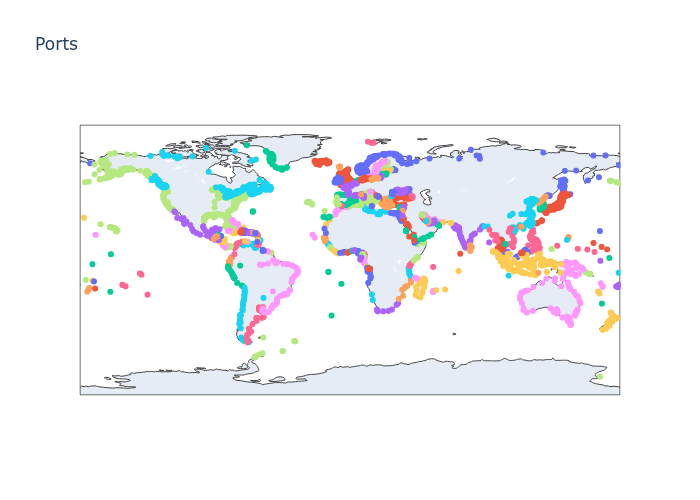
\includegraphics[width = \textwidth]{WPI.png}
\end{figure}

\begin{itemize}
    \item shapefile @ /src/data/WPI
\end{itemize}

\end{frame}

%------------------------------------------------------

\section{Code}

%------------------------------------------------------

\begin{frame}
\frametitle{Linking}

$$ MRV \xleftrightarrow{IMO \#} WFR \xleftrightarrow{MMSI} AIS $$

\begin{figure}
    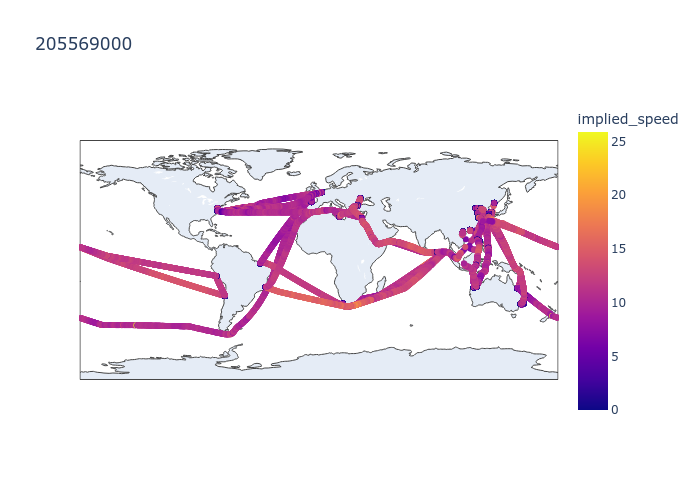
\includegraphics[width = 0.9\textwidth]{205569000_implied_speed.png}
    \caption{Olmer et al. 2017}
\end{figure}

\end{frame}

%------------------------------------------------------

\begin{frame}
\frametitle{Code}
\begin{itemize}
    \item Tracking data is currently a 20GB+ set of parquet files
    \item Divided into separate files ('partitions') to allow for larger-than-memory processing
    \item Each partition contains all observations of a given mmsi and is sorted by date
\end{itemize}

\begin{itemize}
    \item Python
    \begin{itemize}
        \item Dask
        \begin{itemize}
            \item Allows cluster computing / parellelization
            \item Operations are lazy
            \item Use dd.map.partition() to operate on each partition as a Pandas dataframe
        \end{itemize}
        \item Pandas
    \end{itemize}
    \item R (tidyverse)
\end{itemize}

\end{frame}

%------------------------------------------------------

\begin{frame}
\frametitle{Matching MRV and AIS}

\begin{itemize}
    \item MRV reports annual fuel consumption for 'trips' in and out of 'EU'
    \item Need to identify these trips in the tracking data:
    \begin{itemize}
        \item Trip: a voyage with at least one port call within an EU territory
        \item Port call: loading or unloading (not refuelling for example)
        \item EU territory (Continental EU countries plus Norway, Icelancd (minus UK after 2020) plus territories)
    \end{itemize}
\end{itemize}

\vfill

Steps:
\begin{enumerate}
    \item Detect port calls
    \item Number trips
    \item Filter EU trips
    \item Aggregate variables of interest
\end{enumerate}

\end{frame}

%------------------------------------------------------

\end{document}
